\chapter{Diseño e Implementación} % Main chapter title

\label{Chapter3} % Change X to a consecutive number; for referencing this chapter elsewhere, use \ref{ChapterX}
\definecolor{mygreen}{rgb}{0,0.6,0}
\definecolor{mygray}{rgb}{0.5,0.5,0.5}
\definecolor{mymauve}{rgb}{0.58,0,0.82}

\lstset{ %
  backgroundcolor=\color{white},   % choose the background color; you must add \usepackage{color} or \usepackage{xcolor}
  basicstyle=\footnotesize,        % the size of the fonts that are used for the code
  breakatwhitespace=false,         % sets if automatic breaks should only happen at whitespace
  breaklines=true,                 % sets automatic line breaking
  captionpos=b,                    % sets the caption-position to bottom
  commentstyle=\color{mygreen},    % comment style
  deletekeywords={...},            % if you want to delete keywords from the given language
  %escapeinside={\%*}{*)},          % if you want to add LaTeX within your code
  %extendedchars=true,              % lets you use non-ASCII characters; for 8-bits encodings only, does not work with UTF-8
  %frame=single,	                   % adds a frame around the code
  keepspaces=true,                 % keeps spaces in text, useful for keeping indentation of code (possibly needs columns=flexible)
  keywordstyle=\color{blue},       % keyword style
  language=[ANSI]C,					% the language of the code
  %otherkeywords={*,...},           % if you want to add more keywords to the set
  numbers=left,                    % where to put the line-numbers; possible values are (none, left, right)
  numbersep=5pt,                   % how far the line-numbers are from the code
  numberstyle=\tiny\color{mygray}, % the style that is used for the line-numbers
  rulecolor=\color{black},         % if not set, the frame-color may be changed on line-breaks within not-black text (e.g. comments (green here))
  showspaces=false,                % show spaces everywhere adding particular underscores; it overrides 'showstringspaces'
  showstringspaces=false,          % underline spaces within strings only
  showtabs=false,                  % show tabs within strings adding particular underscores
  stepnumber=1,                    % the step between two line-numbers. If it's 1, each line will be numbered
  stringstyle=\color{mymauve},     % string literal style
  tabsize=2,	                   % sets default tabsize to 2 spaces
  title=\lstname,                   % show the filename of files included with \lstinputlisting; also try caption instead of title
  morecomment=[s]{/*}{*/}%
}


%----------------------------------------------------------------------------------------
%	SECTION 1
%----------------------------------------------------------------------------------------
\section{Módulos del sistema de hardware}
 
En el presente capitulo se realiza una explicación detallada de los módulos del hardware, tecnologías usadas, y el diseño e implementación del firmware.


\subsection{Hardware}

En esta sección se explican todos los módulos de hardware que componen el prototipo del proyecto.

En la figura \ref{fig:Hierarchy} se puede observar la jerarquia del diagrama esquemático de todo el hardware.

\begin{figure}[h]
	\centering
	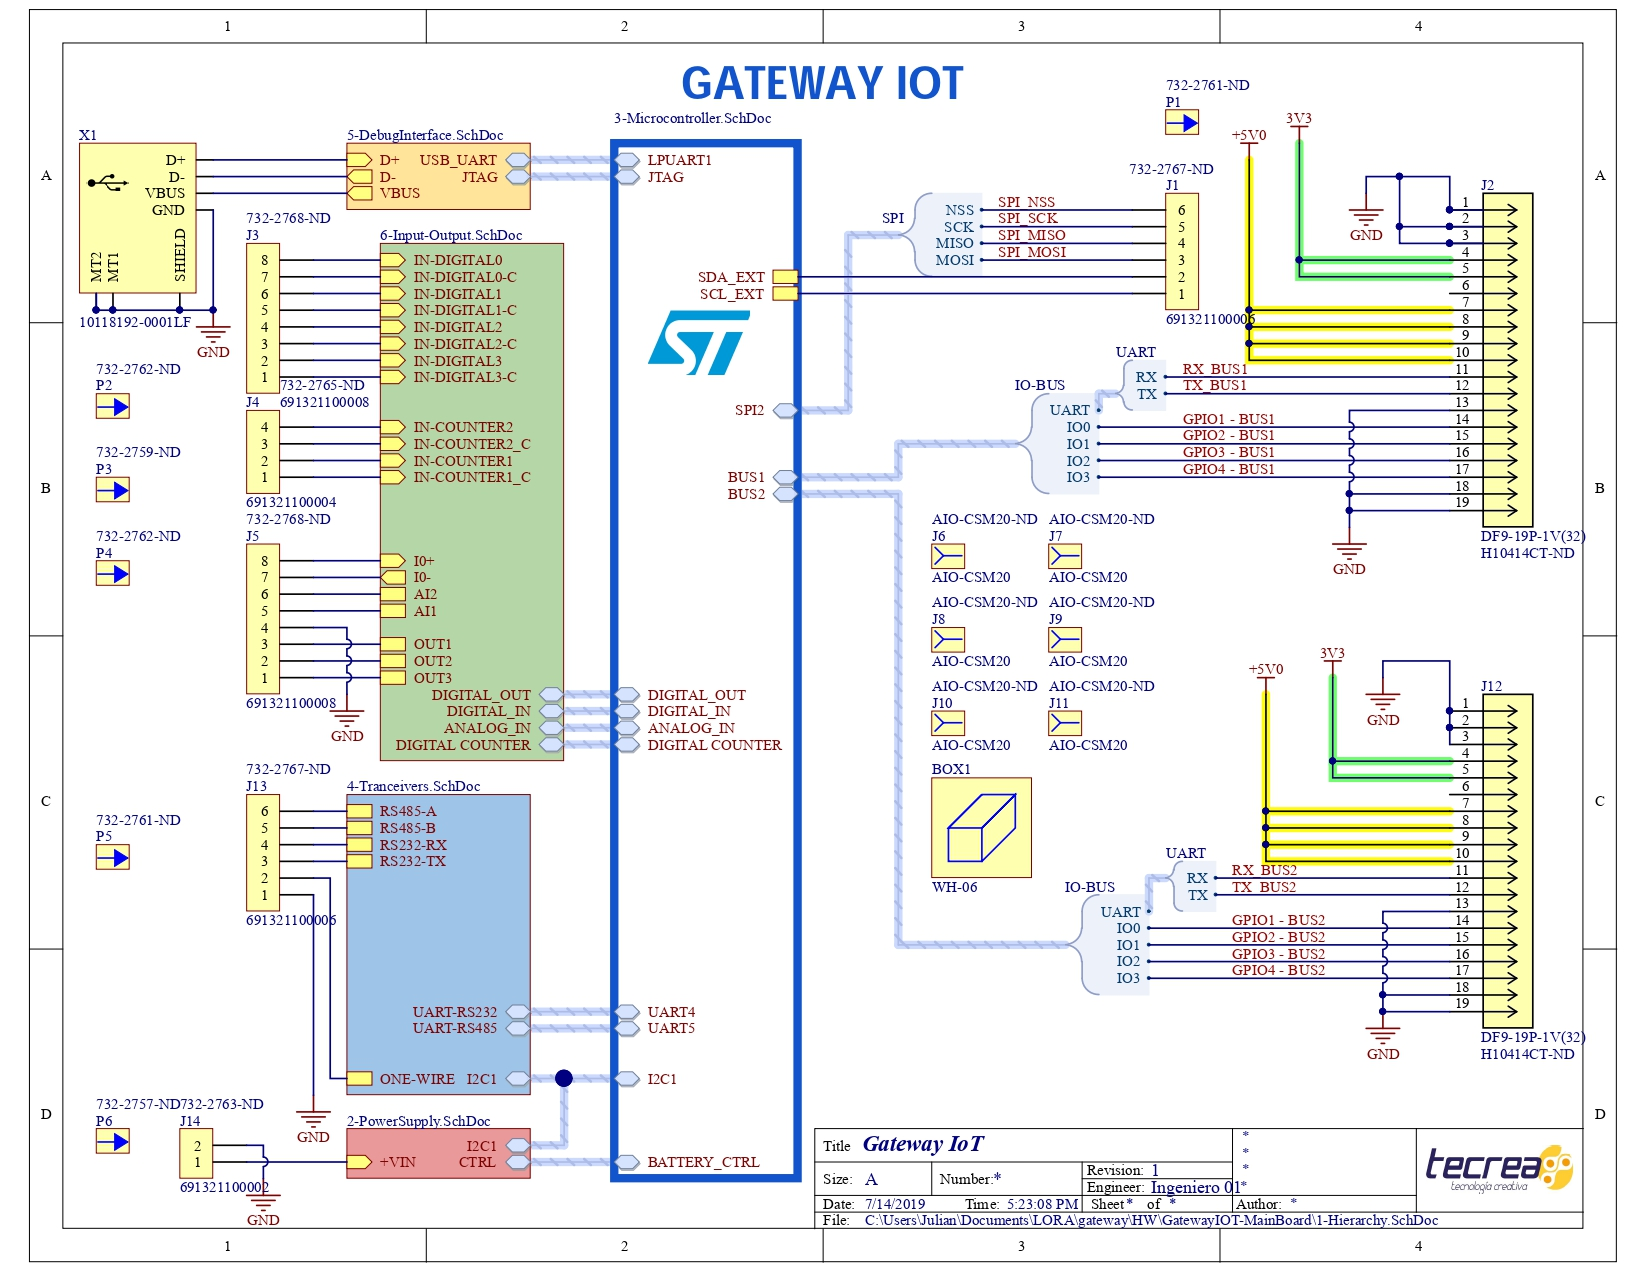
\includegraphics[scale=.55]{./Figures/Hierarchy.jpg}
	\caption{Jerarquia del hardware.}
	\label{fig:Hierarchy}
\end{figure}

\subsubsection{Microcontrolador:}

\begin{itemize}
    \item \textit{Ultra low power} ARM Cortex\textregistered-M4  CPU with FPU
    \item  SRAM 256 KB
    \item  Flash 1M
    \item 30 nA \textit{Shutdown mode (5 wakeup pins)}
    \item 120 nA \textit{Standby mode (5 wakeup pins)}
    \item 420 nA \textit{Standby mode with RTC}
   \item 3x I2C FM+(1 Mbit/s), SMBus/PMBus 
   \item 6x USARTs
   \item 3x SPIs
   \item 14-\textit{channel DMA controller}
    \item 16 x \textit{ timers}: 2 x 16-bit \textit{advanced motor-control}, 2 x 32-bit and 5 x 16-bit \textit{general purpose}, 2x 16-bit \textit{basic}, 2x \textit{low-power} 16-bit \textit{timers (available in Stop mode)}, 2x \textit{watchdogs, SysTick timer}
    \item \textit{Up to 114 fast I/Os, most 5 V-tolerant, up to 14 I/Os with independent supply down to 1.08 V}
\end{itemize}



\subsubsection{Modulo Sigfox}
El módulo para la comunicación Sigfox desarrollado por la empresa WISOL, opera en 2 zonas con frecuencia distinta, la cual puede ser configurable por software.
\begin{itemize}
    \item WISOL WSSFM11R2D \protect\footnotemark
    \item \textit{RF Frecuency} RC2 transmisión 902.2 MHz.
    \item \textit{RF Frecuency} RC2 recepción 905.2 MHz.
    \item \textit{RF Frecuency} RC4 transmisión 920.8 MHz.
    \item \textit{RF Frecuency} RC4 recepción 922.3 MHz.
    \item potencia de Transmisión 22.5 dBm.
    \item 2.5 uA en modo \textit{sleep}.
\end{itemize}
\footnotetext{\url{https://usermanual.wiki/WISOL/SFM11R2D}}

En la figura \ref{fig:SIGFOX_SCH} se observa el diagrama esquemático del hardware asociado al modulo Sigfox.

\begin{figure}[h]
	\centering
	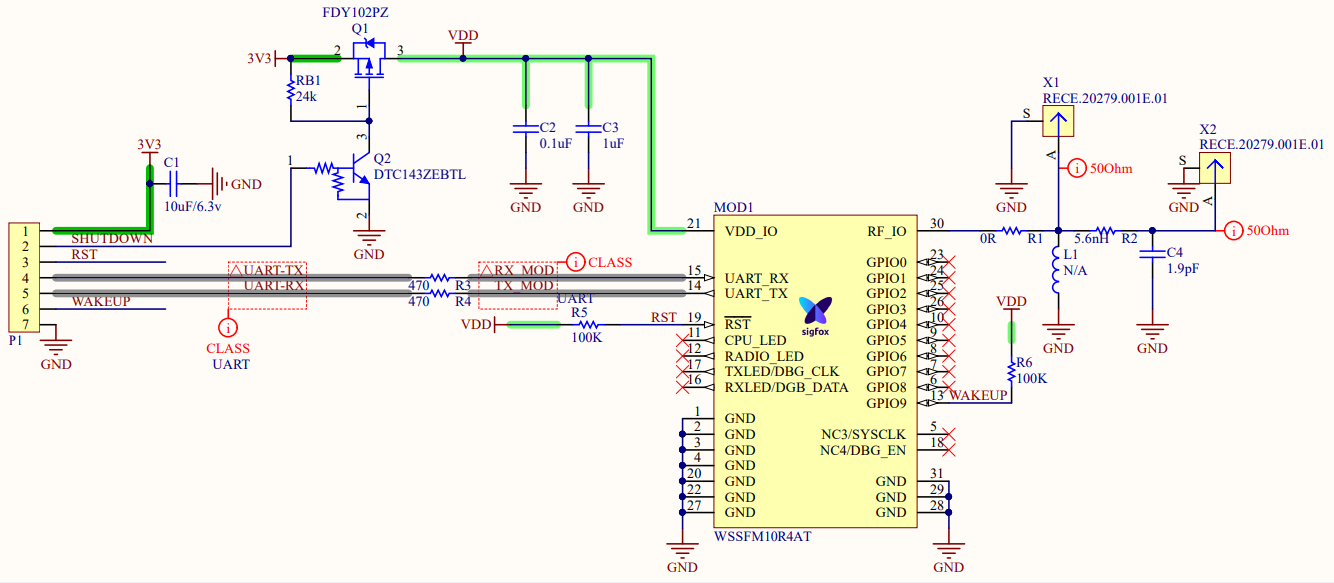
\includegraphics[scale=.4]{./Figures/SIGFOX_SCH.PNG}
	\caption{Esquemático módulo Sigfox.}
	\label{fig:SIGFOX_SCH}
\end{figure}

\subsubsection{Modulo Lora}
El módulo para la comunicación LoRa, es fabricado por la empresa  Microchip Technology.
\begin{itemize}
    \item  RN2903 \protect\footnotemark  clase A.
    \item Opera en la banda de frecuencia de 915 MHz
    \item modulación FSK, GFSK.
    \item 1.3 uA en modo \textit{sleep}.
    \item Potencia de Transmisión ajustable hasta 18.5 dBm.
\end{itemize}
\footnotetext{\url{http://ww1.microchip.com/downloads/en/DeviceDoc/50002390E.pdf}}

En la figura \ref{fig:lORA_SCH} se observa el diagrama esquemático del hardware asociado al módulo LoRa.

\begin{figure}[h]
	\centering
	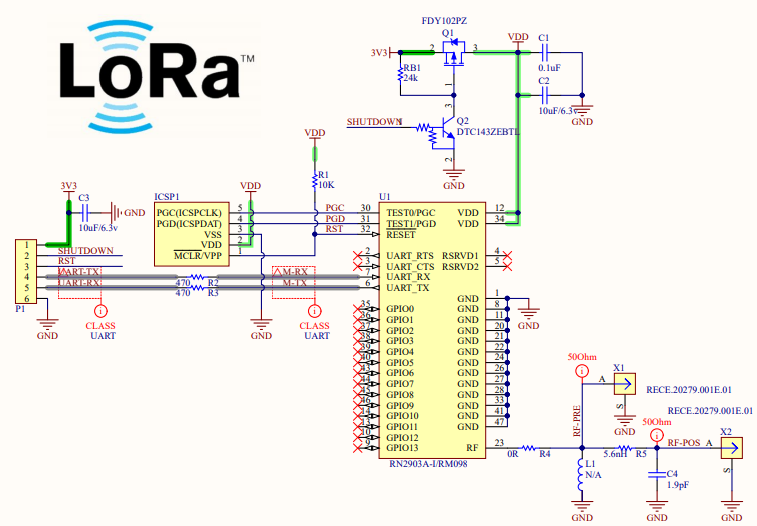
\includegraphics[scale=.55]{./Figures/lORA_SCH.PNG}
	\caption{Esquemático módulo LoRa.}
	\label{fig:lORA_SCH}
\end{figure}

Como el dispositivo esta enfocado al IoT, se garantizo desde la etapa de diseño que los módulos de las dos tecnologías consumieran lo mínimo posible en modo de bajo consumo, por lo que se implemento interruptores con transistores MOSFET (\textit{Metal-oxide-semiconductor Field-effect transistor})en la alimentación principal de cada integrado.

\subsubsection{Entradas analógicas}

En la figura \ref{fig:inputanalog} se puede observar el diagrama esquemático de las entradas analógicas, los valores de las resistencias se escogieron de acuerdo a los niveles de tensión y de corriente de las entradas( 0-5VDC, 0-10VDC, 4-20mA) y el máximo voltaje permitido por el microcontrolador 3.3V. Todas las entradas analógicas tiene amplificadores en modo seguidor para acoplar impedancias y diodos TVS a la salida para garantizar los niveles de tensión máximo (3.3VDC).

\begin{figure}[h]
	\centering
	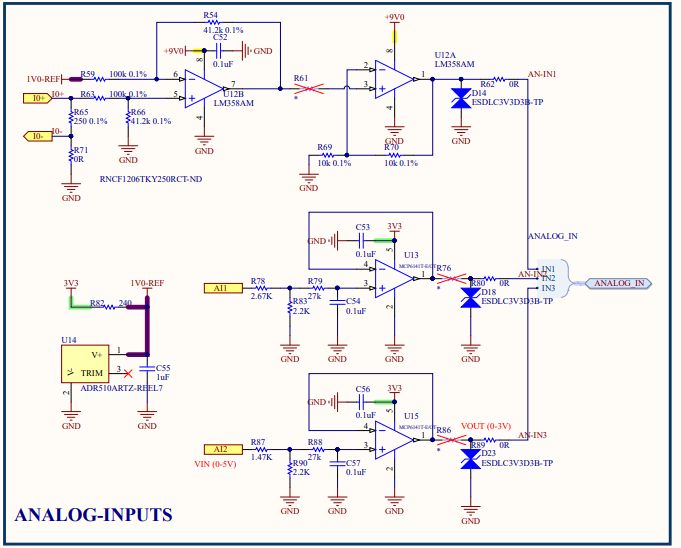
\includegraphics[scale=.65]{./Figures/inputanalog.PNG}
	\caption{Esquemático entradas analógicas.}
	\label{fig:inputanalog}
\end{figure}

\subsubsection{Entradas digitales}

En la figura \ref{fig:digitalinputs} se puede observar el diagrama esquemático de las entradas digitales, estas se encuentran opto-aisladas y funcionan con niveles de voltaje entre 3.3VDC a 24VDC.

\begin{figure}[h]
	\centering
	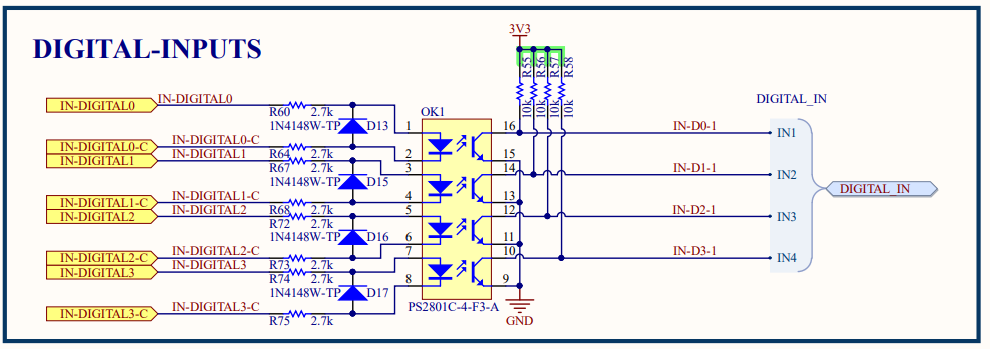
\includegraphics[scale=.45]{./Figures/digitalinputs.PNG}
	\caption{Esquemático entradas analógicas.}
	\label{fig:digitalinputs}
\end{figure}
% Se puede agregar código o pseudocódigo dentro de un entorno lstlisting con el siguiente código:

% \begin{verbatim}
% \begin{lstlisting}[caption= "un epígrafe descriptivo"]

% 	las líneas de código irían aquí...
	
% \end{lstlisting}
% \end{verbatim}

% A modo de ejemplo:

% \begin{lstlisting}[caption=Pseudocódigo del lazo principal de control.]  % Start your code-block

% #define MAX_SENSOR_NUMBER 3
% #define MAX_ALARM_NUMBER  6
% #define MAX_ACTUATOR_NUMBER 6

% uint32_t sensorValue[MAX_SENSOR_NUMBER];		
% FunctionalState alarmControl[MAX_ALARM_NUMBER];	//ENABLE or DISABLE
% state_t alarmState[MAX_ALARM_NUMBER];						//ON or OFF
% state_t actuatorState[MAX_ACTUATOR_NUMBER];			//ON or OFF

% void vControl() {

% 	initGlobalVariables();
	
% 	period = 500 ms;
		
% 	while(1) {

% 		ticks = xTaskGetTickCount();
		
% 		updateSensors();
		
% 		updateAlarms();
		
% 		controlActuators();
		
% 		vTaskDelayUntil(&ticks, period);
% 	}
% }
% \end{lstlisting}


%-------------
%
%--------------

Antena :
\subsection{Sintonización y verificación de la antena.}

\subsection{Desarrollo de la capa de manejadores de dispositivos(\textit{driver}).}

\subsection{Diseño del firmware}

\subsection{Implementación del firmware  y herramientas a usar.}


